

\chapter{Outros sistemas de coordenadas}\label{cap_osc}
\thispagestyle{fancy}

Neste capítulo, vamos introduzir outros sistemas de coordenadas no plano e no espaço tridimensional.

\section{Sistema de coordenadas polares}\label{cap_osc_scp}

No plano, o sistema de coordenadas polares é definido por um ponto de origem (chamado de \emph{polo}) e um eixo orientado $Ox$ (chamado de \emph{eixo polar}). Veja a Figura \ref{fig:osc_scp}.

\begin{figure}[H]
  \centering
  \includegraphics[width=0.6\textwidth]{cap_osc/dados/fig_osc_scp/fig}
  \caption{Sistema de coordenadas polares.}
  \label{fig:osc_scp}
\end{figure}

Neste sistema, um ponto $P$ de coordenadas polares ${\color{blue}P=(r, \theta)}$ é tal que ${\color{blue}|OP| = r}$ (i.e. a distância do polo ao ponto é $r$) e ${\color{blue}\theta}$ é o ângulo de $Ox$ com $OP$, medido positivamente no sentido anti-horário.

\begin{ex}
  Na Figura \ref{fig:ex_osc_scp}, temos a representação dos pontos ${\color{blue}P=(2\sqrt{2}, \frac{\pi}{4})}$, ${\color{red}A=(2, \frac{2\pi}{3})}$ e ${\color{orange}B=(\sqrt{2}, \frac{5\pi}{4})}$ no sistema de coordenadas polares.

\begin{figure}[H]
  \centering
  \includegraphics[width=0.6\textwidth]{cap_osc/dados/fig_ex_osc_scp/fig}
  \caption{Sistema de coordenadas polares.}
  \label{fig:ex_osc_scp}
\end{figure}  
\end{ex}

\begin{obs}
  Por convenção, as coordenadas polares $(r, \pi + \theta) = (-r, \theta)$, $r>0$. Por exemplo, $B=(\sqrt{2}, \frac{5\pi}{4}) = (-\sqrt{2}, \frac{\pi}{4})$. Veja na Figura \ref{fig:ex_osc_scp}.
\end{obs}

\subsection{Coordenadas cartesianas x polares}

Aqui, vamos estudar como podemos converter as coordenadas de um ponto $P$ de coordenadas cartesianas para coordenadas polares e vice-versa. Vamos denotar as coordenadas cartesianas do ponto $P$ por $P=(x_P, y_P)$ e suas coordenadas polares por $P=(r, \theta)$. Veja a Figura \ref{fig:osc_ccxcp}.

\begin{figure}[H]
  \centering
  \includegraphics[width=0.5\textwidth]{cap_osc/dados/fig_osc_ccxcp/fig}
  \caption{Sistema de coordenadas polares.}
  \label{fig:osc_ccxcp}
\end{figure}  

Na Figura \ref{fig:osc_ccxcp}, vamos nos concentrar no triângulo retângulo de vértices $O$, $(x_P, 0)$ e $P$. Das relações trigonométricas e do teorema de Pitágoras, temos que
\begin{gather}
  \cos\theta = \frac{x_P}{r} \\
  \sen\theta = \frac{y_P}{r} \\
  r^2 = x_P^2 + y_P^2 \\
  \tg\theta = \frac{y_P}{x_P}
\end{gather}
ou, equivalentemente,
\begin{gather}
  {\color{blue}x_P = r\cos\theta} \\
  {\color{blue}y_P = r\sen\theta} \\
  {\color{blue}r = \sqrt{x_P^2 + y_P^2 }} \\
  {\color{blue}\theta = \arc\tg\left(\frac{y_P}{x_P}\right)}
\end{gather}

\begin{ex}
  Vejamos os seguintes casos:
  \begin{enumerate}
  \item[a)] Conversão de $P=(2\sqrt{2}, \frac{\pi}{4})$ em coordenadas polares para coordenadas cartesianas.

    No caso de $P=(2\sqrt{2}, \frac{\pi}{4}$ temos $r=2\sqrt{2}$ e $\theta = \frac{\pi}{4}$. Desta forma, as coordenadas cartesianas de $P=(x,y)$ são dadas por
    \begin{align}
      x &= r\cos\theta \\
        &= 2\sqrt{2}\cos\frac{\pi}{4}\\
        &= 2\sqrt{2}\cdot \frac{\sqrt{2}}{2}\\
        &= 2\\
      ~&~\nonumber\\
      y &= r\sen\theta\\
        &= 2\sqrt{2}\sen\frac{\pi}{4}\\
        &= 2\sqrt{2}\cdot\frac{\sqrt{2}}{2}\\
        &= 2
    \end{align}
    Logo, $P=(2,2)$ em coordenadas cartesianas. Veja a Figura \ref{fig:ex_osc_scp}.

  \item[b)] Conversão de $B=(-\sqrt{3}, -1)$ de coordenadas cartesianas para coordenadas polares. Neste caso, temos $x=-\sqrt{3}$ e $y=-1$ e
    \begin{align}
      r &= \sqrt{x^2 + y^2} \\
        &= \sqrt{(-\sqrt{3})^2 + (-1)^2}\\
        &= \sqrt{4} \\
        &= 2\\
      ~&~\nonumber\\
      \theta &= \arc\tg\left(\frac{y}{x}\right)\\
        &= \arc\tg\left(\frac{-1}{-\sqrt{3}}\right)\\
        &= \arc\tg\left(\frac{\sqrt{3}}{3}\right)\\
        &= \frac{7\pi}{6}.
    \end{align}
    Desta forma, temos que $P=(2, \frac{7\pi}{6})$ em coordenadas polares. Ou, equivalentemente, $P=(-2, \frac{\pi}{6})$.
  \end{enumerate}
\end{ex}

\subsubsection{Equação de reta que passa pela origem}

Em coordenadas polares, uma reta que passa pela origem e tem ângulo de declividade $\theta_0$ tem equação
\begin{equation}
  \theta = \theta_0,
\end{equation}
com $r\in\mathbb{R}$.

\begin{ex}
  Seja a reta $y=x$ em coordenadas cartesianas. Em coordenadas polares, a equação desta reta é
  \begin{equation}
    \theta = \frac{\pi}{4}.
  \end{equation}
\end{ex}

\subsubsection{Equação de circunferência com centro na origem}

Em coordenadas polares, a circunferência com centro na origem e raio $r_0$ tem equação
\begin{equation}
  r = r_0.
\end{equation}

\begin{ex}
  Seja a circunferência $x^2 + y^2 = 4$ em coordenadas cartesianas. Em coordenadas polares, a equação desta circunferência é
  \begin{equation}
    r = 2.
  \end{equation}
\end{ex}

\subsection{Exercícios resolvidos}

\begin{exeresol}
  Obtenha duas representações em coordenadas polares do ponto $A=(-1,0)$ dado em coordenadas cartesianas.
\end{exeresol}
\begin{resol}
  O ponto $A=(-1, 0)$ tem coordenadas cartesianas $x=-1$ e $y=0$. Para converter em coordenadas polares $A=(r, \theta)$, podemos usar
  \begin{align}
    r^2 &= x^2 + y^2 \\
    r^2  &= 1^2 + 0^2 \\
    r  &= \pm 1
  \end{align}
  e
  \begin{align}
    \theta &= \arc\tg\left(\frac{y}{x}\right) \\
           &= \arc\tg\left(0\right) \\
           &= \pi\text{ ou }0. 
  \end{align}
  Ou seja, em coordenadas polares, temos as representações $A=(1, \pi)$ ou $A=(-1,0)$.
\end{resol}

\begin{exeresol}
  Obtenha a representação em coordenadas cartesianas do ponto $B=(2, \frac{\pi}{2})$ dado em coordenadas polares.
\end{exeresol}
\begin{resol}
  O ponto $B=(2, \frac{\pi}{2})$ tem coordenadas polares $r=2$ e $\theta=\frac{\pi}{2}$. Para converter em coordenadas cartesianas $B=(x, y)$, podemos usar
  \begin{align}
    x &= r\cos\theta \\
      &= 2\cos\frac{\pi}{2} \\
      &= 0
  \end{align}
  e
  \begin{align}
    y &= r\sen\theta \\
      &= 2\sen\frac{\pi}{2} \\
      &= 2 
  \end{align}
  Ou seja, em coordenadas cartesianas, temos a representação $B=(0, 2)$.
\end{resol}

\subsection*{Exercícios}

\begin{exer}
  Obtenha uma representação em coordenadas polares dos seguintes pontos dados em coordenadas cartesianas:
  \begin{enumerate}[a)]
  \item $A=(-3, 3)$
  \item $B=(\frac{3}{2}, \frac{\sqrt{3}}{2})$
  \item $C=(\frac{3}{2}, -\frac{\sqrt{3}}{2})$
  \end{enumerate}
\end{exer}
\begin{resp}
  a) $A=(3\sqrt{2}, \frac{3\pi}{4})$; b) $B = (\sqrt{3}, \frac{\pi}{6})$; c) $C=(\sqrt{3}, \frac{11\pi}{6})$
\end{resp}

\begin{exer}
  Obtenha uma representação em coordenadas cartesianas dos seguintes pontos dados em coordenadas polares:
  \begin{enumerate}[a)]
  \item $A=(2, \frac{\pi}{6})$
  \item $B=(1, \frac{5 \pi}{6})$
  \item $C=(-2, \frac{3\pi}{4})$
  \end{enumerate}
\end{exer}
\begin{resp}
  a) $A=(\sqrt{3}, 1)$; b) $B = (-\frac{\sqrt{3}}{2}, \frac{1}{2})$; c) $C=(\sqrt{2}, -\sqrt{2})$
\end{resp}

\begin{exer}
  Considere a reta de equação $x = 0$ em coordenadas cartesianas. Escreva a equação desta reta em coordenadas polares.
\end{exer}
\begin{resp}
  $\theta = \frac{\pi}{2}$
\end{resp}

\begin{exer}
  Considere a reta de equação $\theta = \frac{3\pi}{4}$ em coordenadas polares. Escreva a equação desta reta em coordenadas cartesianas.
\end{exer}
\begin{resp}
  $y = -x$
\end{resp}

\begin{exer}
  Considere a circunferência de equação $x^2 + y^2 = 1$ em coordenadas cartesianas. Escreva a equação desta circunferência em coordenadas polares.
\end{exer}
\begin{resp}
  $r = 1$
\end{resp}

\begin{exer}
  Considere a circunferência de equação $r = \sqrt{2}$ em coordenadas polares. Escreva a equação desta circunferência em coordenadas cartesianas.
\end{exer}
\begin{resp}
  $x^2 + y^2 = 2$
\end{resp}
